\subsection{huffman e shannon-fano-elias}
% http://www2.cs.uregina.ca/~mouhoubm/=postscript/=c3620/final_02F.pdf
% slide 549 - Example (distribuição diádica)

\begin{questions}
\question{
Você deverá criar o códigos de Huffman e Shannon-Fano-Elias para comprimir um texto
com as seguintes características. O texto possui apenas os símbolos `a', `b', `c' e `d'.
Estes símbolos aparecem 50, 100, 25 e 25 vezes, respectivamente. Suponha que inicialmente
o seu texto está codificado em ASCII (8 bits por símbolo). Faça o que se pede.

\begin{parts}
\part Calcule a entropia da fonte.

\part Calcule o tamanho original do texto.

\part Encontre o código de Huffman para este texto.

\part Encontre o código de Shannon-Fano-Elias para este texto.

\part Calcule a eficiência dos códigos.

\part Calcule o tamanho do arquivo codificado com cada um dos dois códigos.

\part Faça a árvore para ambos códigos.

\part Caracterize os códigos quanto aos seguintes aspectos: singularidade,
univocidade, instantaneidade.

\part Verifique quais dos dois códigos satisfaz a desigualdade de Kraft. 

\end{parts}
}


\begin{solution}
\begin{parts}
\part 
  A estimativa da distribuição da fonte é 
  \begin{equation}
  p = \begin{pmatrix} \frac{1}{4} & \frac{1}{2} & \frac{1}{8} & \frac{1}{8} \end{pmatrix} 
  \end{equation}


  \begin{eqnarray}
  H &=& - \sum_p p_i \log p_i \\
    &=& - \frac{1}{4} \log \frac{1}{4} - \frac{1}{2} \log \frac{1}{2} - \frac{1}{8} \log \frac{1}{8} - \frac{1}{8} \log \frac{1}{8} \\
    &=& - \frac{1}{4} (-2) - \frac{1}{2} (-1) - 2 \times \frac{1}{8} (-3) \\
    &=& \frac{1}{2} + \frac{1}{2} + \frac{3}{4} = \frac{7}{4}
  \end{eqnarray} 

\begin{lstlisting}[language=Octave]
>> f=[50 100 25 25];
>> p=f./sum(f);
>> entropy(p)
ans =  1.7500
\end{lstlisting}



\part 

  \begin{equation}
  (50 + 100 + 25 + 25) \times 8 = 200 \times 8 = 1600 \text{ bits}.
  \end{equation}

\part 

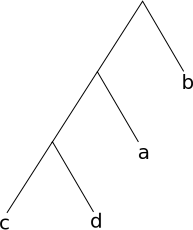
\includegraphics[width=0.15\textwidth]{../images/hufftree.pdf}

\begin{lstlisting}[language=Octave]
>> dict = huffmandict({'a','b','c','d'}, p)
dict = 
{
  [1,1] =  0   1
  [1,2] =  1
  [1,3] =  0   0   0
  [1,4] =  0   0   1
}
\end{lstlisting}
$El_{\text{huffman}} = 0.5 \time 1 + 0.25 \times 2 + 0.125 \times 3 + 0.125 \times 3 = 1.75$


\part
\ 
 
  \begin{tabular}{lllllll}
  $x$ & $p(x)$ & $F(x)$ & $\overline{F}(x)$       & $\overline{F}(x)$ (binário) & $l(x)$ & palavra código \\ \hline
   a   & 0.25   & 0.25   & 0.125           & 0.001                 & 3     & 001   \\
   b   & 0.5    & 0.75   & 0.5             & 0.10                  & 2     & 10    \\
   c   & 0.125  & 0.875  & 0.8125          & 0.1101                & 4     & 1101  \\
   d   & 0.125  & 1.0    & 0.9375          & 0.1111                & 4     & 1111
  \end{tabular}

   $El = 2.75$ bits 

\part 

  \begin{equation}
  \text{eficiência}_{\text{huffman}} = \frac{1.75}{1.75} = 1
  \end{equation}

  \begin{equation}
  \text{eficiência}_{\text{shannon-fano}} = \frac{1.75}{2.75} = \frac{7}{4} \times \frac{4}{11} = \frac{7}{11} = 0.64
  \end{equation}


\part 

  Huffman
  \begin{equation}
  50 \times 2 + 100 \times 1 + 25 \times 3 + 25 \times 3 = 350 \text{ bits}
  \end{equation}

  Shannon-Fano-Elias
  \begin{equation}
  50 \times 3 + 100 \times 2 + 25 \times 4 + 25 \times 4 = 550 \text{ bits}
  \end{equation}


Árvore de Huffman: $((a,(c,d)),b)$.

 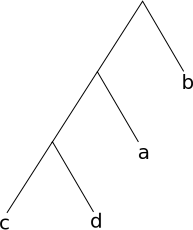
\includegraphics[width=0.15\textwidth]{../images/hufftree.pdf}

\vspace{0.2cm}

Árvore de Shannon-Fano-Elias: 

 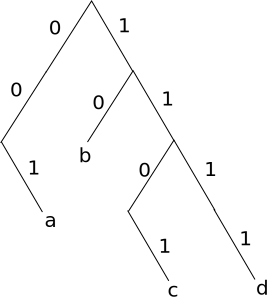
\includegraphics[width=0.2\textwidth]{../images/shannofano.pdf}

\part 

Ambos códigos são códigos de prefixo (instantâneos), por conseguinte, são singulares e unívocos.

\part 

Ambos códigos são códigos de prefixo, devem portanto satisfazer a desigualdade de Kraft.

Vamos verificar.

O código de Huffman possui comprimentos $l = (2, 1, 3, 3)$.
\begin{eqnarray}
\sum_i 2^{-l_i} &=& 2^{-2} + 2^{-1} + 2^{-3} + 2^{-3} \\
                &=& \frac{1}{4} + \frac{1}{2} + \frac{1}{8} + \frac{1}{8} = 1 \leq 1.
\end{eqnarray}

O código de Shannon-Fano-Eliasn possui comprimentos $l = (3, 2, 4, 4)$.
\begin{eqnarray}
\sum_i 2^{-l_i} &=& 2^{-3} + 2^{-2} + 2^{-4} + 2^{-4} \\
                &=& \frac{1}{8} + \frac{1}{4} + \frac{1}{16} + \frac{1}{16} = \frac{1}{2} \leq 1.
\end{eqnarray}
 


\end{parts}
\end{solution}
\end{questions}
